% Options for packages loaded elsewhere
% Options for packages loaded elsewhere
\PassOptionsToPackage{unicode}{hyperref}
\PassOptionsToPackage{hyphens}{url}
\PassOptionsToPackage{dvipsnames,svgnames,x11names}{xcolor}
%
\documentclass[
  english,
  11pt,
]{article}
\usepackage{xcolor}
\usepackage[margin=25mm]{geometry}
\usepackage{amsmath,amssymb}
\setcounter{secnumdepth}{-\maxdimen} % remove section numbering
\usepackage{iftex}
\ifPDFTeX
  \usepackage[T1]{fontenc}
  \usepackage[utf8]{inputenc}
  \usepackage{textcomp} % provide euro and other symbols
\else % if luatex or xetex
  \usepackage{unicode-math} % this also loads fontspec
  \defaultfontfeatures{Scale=MatchLowercase}
  \defaultfontfeatures[\rmfamily]{Ligatures=TeX,Scale=1}
\fi
\usepackage{lmodern}
\ifPDFTeX\else
  % xetex/luatex font selection
\fi
% Use upquote if available, for straight quotes in verbatim environments
\IfFileExists{upquote.sty}{\usepackage{upquote}}{}
\IfFileExists{microtype.sty}{% use microtype if available
  \usepackage[]{microtype}
  \UseMicrotypeSet[protrusion]{basicmath} % disable protrusion for tt fonts
}{}
\makeatletter
\@ifundefined{KOMAClassName}{% if non-KOMA class
  \IfFileExists{parskip.sty}{%
    \usepackage{parskip}
  }{% else
    \setlength{\parindent}{0pt}
    \setlength{\parskip}{6pt plus 2pt minus 1pt}}
}{% if KOMA class
  \KOMAoptions{parskip=half}}
\makeatother
% Make \paragraph and \subparagraph free-standing
\makeatletter
\ifx\paragraph\undefined\else
  \let\oldparagraph\paragraph
  \renewcommand{\paragraph}{
    \@ifstar
      \xxxParagraphStar
      \xxxParagraphNoStar
  }
  \newcommand{\xxxParagraphStar}[1]{\oldparagraph*{#1}\mbox{}}
  \newcommand{\xxxParagraphNoStar}[1]{\oldparagraph{#1}\mbox{}}
\fi
\ifx\subparagraph\undefined\else
  \let\oldsubparagraph\subparagraph
  \renewcommand{\subparagraph}{
    \@ifstar
      \xxxSubParagraphStar
      \xxxSubParagraphNoStar
  }
  \newcommand{\xxxSubParagraphStar}[1]{\oldsubparagraph*{#1}\mbox{}}
  \newcommand{\xxxSubParagraphNoStar}[1]{\oldsubparagraph{#1}\mbox{}}
\fi
\makeatother


\usepackage{longtable,booktabs,array}
\newcounter{none} % for unnumbered tables
\usepackage{calc} % for calculating minipage widths
% Correct order of tables after \paragraph or \subparagraph
\usepackage{etoolbox}
\makeatletter
\patchcmd\longtable{\par}{\if@noskipsec\mbox{}\fi\par}{}{}
\makeatother
% Allow footnotes in longtable head/foot
\IfFileExists{footnotehyper.sty}{\usepackage{footnotehyper}}{\usepackage{footnote}}
\makesavenoteenv{longtable}
\usepackage{graphicx}
\makeatletter
\newsavebox\pandoc@box
\newcommand*\pandocbounded[1]{% scales image to fit in text height/width
  \sbox\pandoc@box{#1}%
  \Gscale@div\@tempa{\textheight}{\dimexpr\ht\pandoc@box+\dp\pandoc@box\relax}%
  \Gscale@div\@tempb{\linewidth}{\wd\pandoc@box}%
  \ifdim\@tempb\p@<\@tempa\p@\let\@tempa\@tempb\fi% select the smaller of both
  \ifdim\@tempa\p@<\p@\scalebox{\@tempa}{\usebox\pandoc@box}%
  \else\usebox{\pandoc@box}%
  \fi%
}
% Set default figure placement to htbp
\def\fps@figure{htbp}
\makeatother



\ifLuaTeX
\usepackage[bidi=basic,shorthands=off]{babel}
\else
\usepackage[bidi=default,shorthands=off]{babel}
\fi
\ifLuaTeX
  \usepackage{selnolig} % disable illegal ligatures
\fi


\setlength{\emergencystretch}{3em} % prevent overfull lines

\providecommand{\tightlist}{%
  \setlength{\itemsep}{0pt}\setlength{\parskip}{0pt}}



 


\makeatletter
\@ifpackageloaded{caption}{}{\usepackage{caption}}
\AtBeginDocument{%
\ifdefined\contentsname
  \renewcommand*\contentsname{Table of contents}
\else
  \newcommand\contentsname{Table of contents}
\fi
\ifdefined\listfigurename
  \renewcommand*\listfigurename{List of Figures}
\else
  \newcommand\listfigurename{List of Figures}
\fi
\ifdefined\listtablename
  \renewcommand*\listtablename{List of Tables}
\else
  \newcommand\listtablename{List of Tables}
\fi
\ifdefined\figurename
  \renewcommand*\figurename{Figure}
\else
  \newcommand\figurename{Figure}
\fi
\ifdefined\tablename
  \renewcommand*\tablename{Table}
\else
  \newcommand\tablename{Table}
\fi
}
\@ifpackageloaded{float}{}{\usepackage{float}}
\floatstyle{ruled}
\@ifundefined{c@chapter}{\newfloat{codelisting}{h}{lop}}{\newfloat{codelisting}{h}{lop}[chapter]}
\floatname{codelisting}{Listing}
\newcommand*\listoflistings{\listof{codelisting}{List of Listings}}
\makeatother
\makeatletter
\makeatother
\makeatletter
\@ifpackageloaded{caption}{}{\usepackage{caption}}
\@ifpackageloaded{subcaption}{}{\usepackage{subcaption}}
\makeatother
\usepackage{bookmark}
\IfFileExists{xurl.sty}{\usepackage{xurl}}{} % add URL line breaks if available
\urlstyle{same}
% fallback for those not using the hyperref driver hyperxmp:
\makeatletter
\@ifundefined{xmpquote}{\newcommand{\xmpquote}[1]{#1}}{}
\makeatother
\hypersetup{
  pdftitle={How the outer vortex fixes pressure at the axis},
  pdflang={en},
  colorlinks=true,
  linkcolor={blue},
  filecolor={Maroon},
  citecolor={Blue},
  urlcolor={Blue},
  pdfcreator={LaTeX via pandoc}}


\title{How the outer vortex fixes pressure at the axis}
\usepackage{etoolbox}
\makeatletter
\providecommand{\subtitle}[1]{% add subtitle to \maketitle
  \apptocmd{\@title}{\par {\large #1 \par}}{}{}
}
\makeatother
\subtitle{D6 stage C: a source-defined input for the inner-profile
solver}
\author{}
\date{2026-09-12}
\begin{document}
\maketitle


\textbf{Pressure at the vortex axis is constrained by the flow outside
it. We now compute that pressure from the paper's prescribed radial
schedule and use it in the inner solver. This supplies a missing input;
the complete joined flow and its first correction remain unfinished.}

The \href{../d6_inner_profile/article.html}{previous study} built a
numerical solver for the leading inner equations. It needed pressure
values along the axis, so it began with a clearly declared analytic test
function. That was enough to test the recurrence, but it left a physical
and mathematical question: where should those pressure values come from
in the paper's construction?

In a swirling flow, radial pressure variation supplies centripetal
acceleration. Once the pressure is fixed at radial infinity, integrating
that balance inward determines the pressure at the axis. We therefore
cannot choose the inner pressure and the exterior swirl independently.

This article follows that dependency. We evaluate the source's pressure
integral, check it against independent calculations, and pass its axial
derivatives to the inner recurrence. The calculation also illustrates
two numerical issues that recur in this project: enormous scale ranges
and the difference between a small equation defect and an accurate
input.

\subsection{Pressure remembers the entire radial
profile}\label{pressure-remembers-the-entire-radial-profile}

The leading radial balance is

\[
\Pi_X=\frac{E^2}{2X}.
\]

With pressure normalized to vanish at radial infinity, the axis value is

\[
\Pi_0(\eta)=-\frac12\int_{-\infty}^{\infty}
E_{\mathrm{id,sched}}(y,\eta)^2\,dy,
\qquad y=\log(X/X_R).
\]

Here \(X\) is the radial similarity coordinate, \(X_R\) is the later
joining scale, and \(\eta\) is the axial similarity parameter. The
logarithmic coordinate removes \(X_R\) from the integral. Moving that
radial scale therefore does not change the axis-pressure datum.

The source allows this integral to use its ideal azimuthal schedule with
certain angular correction bumps omitted: those bumps preserve the total
pressure increment. Their interval lengths and all other transitions
must still be retained. The later heat replacement also has a
compensation that restores the same integral. This lets us compute the
datum before implementing every outer correction.
\href{https://cdn.openai.com/pdf/32d9f210-8b73-45e0-91bc-82a30aef8a9a/navier-stokes.pdf}{OpenAI,
Lemma A.5 and Equations (A.21)--(A.23), pages 133--134; Proposition A.7,
pages 139--140}

\subsection{Use the source's schedule, with declared numerical
choices}\label{use-the-sources-schedule-with-declared-numerical-choices}

The schedule begins with

\[
E=P_*f(\eta)e^{y/10},\qquad
f(\eta)=\frac{1}{1+\eta^2},\qquad y\le0.
\]

That initial branch contributes exactly

\[
\Pi_{0,\mathrm{initial}}=-\frac52P_*^2f^2.
\]

The following intervals change the radial slope, allow the axial flow to
decrease, reserve room for moment corrections, remove the azimuthal
profile's \(\eta\) dependence, and approach the exterior power law. We
implement those intervals in their own local logarithmic coordinates.
The smooth transitions use the function specified in Equation (A.5).
\href{https://cdn.openai.com/pdf/32d9f210-8b73-45e0-91bc-82a30aef8a9a/navier-stokes.pdf}{Appendix
A.2, pages 129--130}

For this numerical schedule we choose \(M_d=2\), \(\lambda=0.02\),
\(h=10^{-9}\), interpolation length \(T_f=100\), and terminal constant
\(c_o=0.01\). We set \(T_d=e^{M_d}+10\) and \(\log P_*=T_d+1\). These
satisfy the source's displayed scalar inequalities, including
\(P_*>e^{T_d}\) and \(h<e^{-T_d}\).

\textbf{They do not certify all the source's ``sufficiently large'' or
``sufficiently small'' choices.} In particular, this study does not
establish the full stress cone or outer moment construction. The
\href{../../code/d6_axis_pressure/parameters.json}{parameter file}
records that distinction alongside every numerical choice.

\begin{figure}

\centering{

\pandocbounded{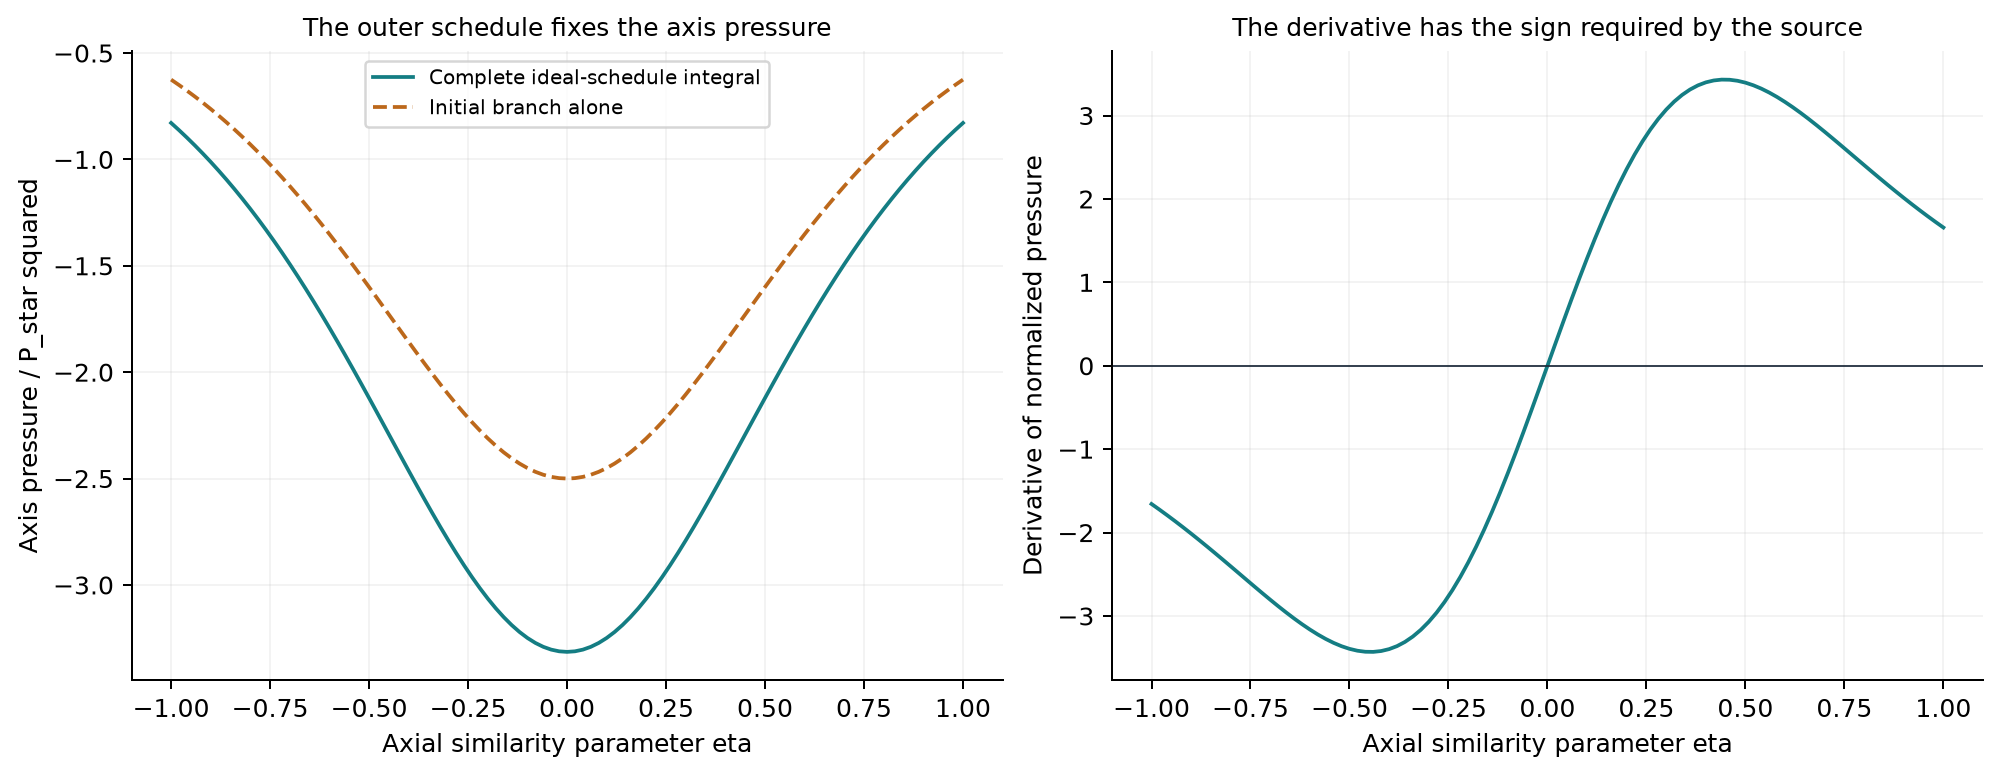
\includegraphics[keepaspectratio,alt={The computed axis pressure is negative and even; its derivative is negative for negative eta and positive for positive eta.}]{figures/01_source_axis_pressure.png}}

}

\caption{\label{fig-pressure}The complete pressure integral and its
exact initial-branch contribution. Pressure is even in eta, and its
derivative has the sign of eta. Both panels use the normalized pressure
Pi0/P\_star squared.}

\end{figure}%

At the center, \(\Pi_0(0)/P_*^2\approx\) \textbf{-3.314622730}.

The initial branch supplies about \textbf{75.4\%} of its magnitude.
Using that branch alone would miss a substantial part of the pressure
datum.

\subsection{Keep small contributions
visible}\label{keep-small-contributions-visible}

For these finite choices, the terminal power law starts near
\(\log_{10}(X/X_R)\approx\) \textbf{537.1}.

Directly storing that radius as an ordinary floating-point number would
overflow. Some late pressure contributions have the opposite problem:
they are too small to store directly in binary64 arithmetic.

We avoid both problems by storing logarithmic radius, logarithmic
amplitudes, and logarithmic pressure contributions. The initial and
infinite final power-law integrals are evaluated analytically. Finite
smooth intervals use Gauss--Legendre quadrature.

\begin{figure}

\centering{

\pandocbounded{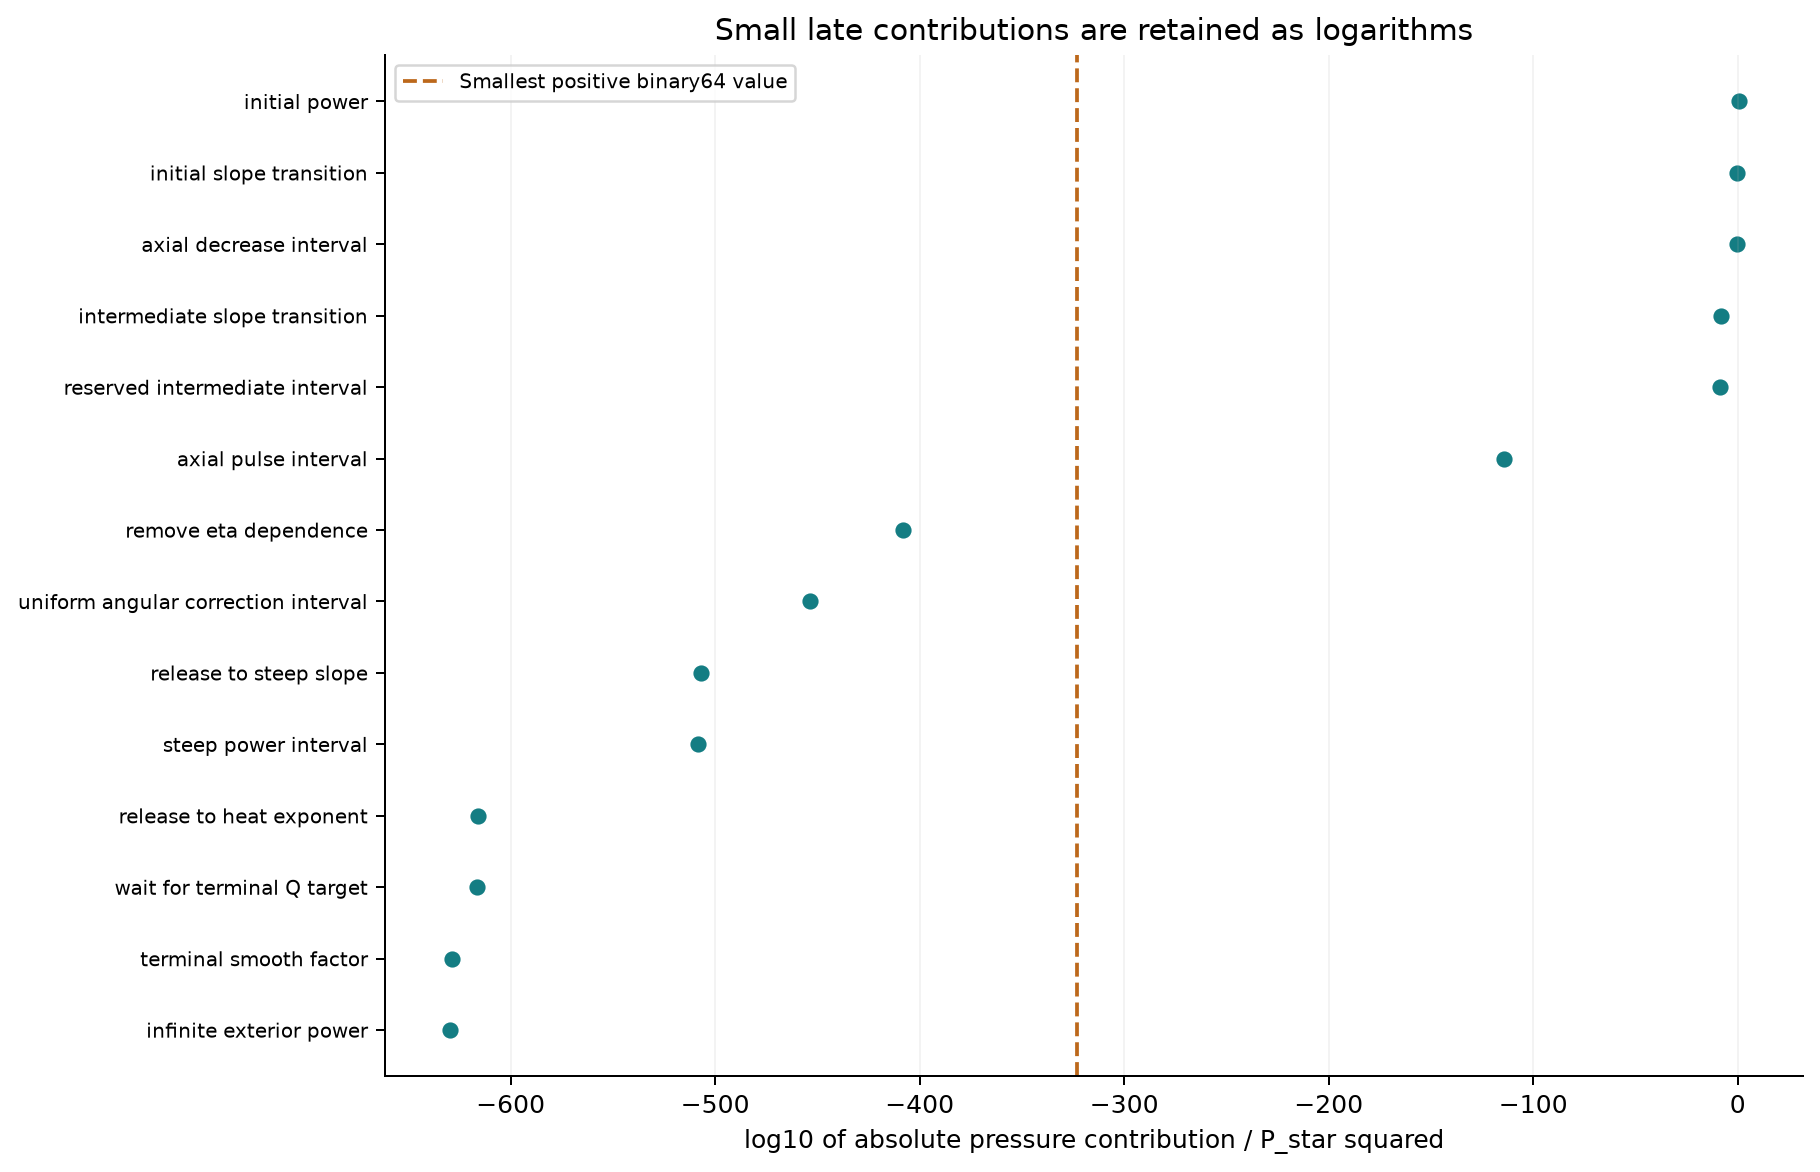
\includegraphics[keepaspectratio,alt={The pressure contributions span over 600 orders of magnitude, with several late intervals below the smallest positive binary64 value.}]{figures/02_pressure_contribution_scales.png}}

}

\caption{\label{fig-scales}Each point is a separate interval's
contribution to the magnitude of Pi0(0)/P\_star squared. Contributions
left of the dashed line cannot be represented as positive binary64
numbers directly, but their logarithms remain available. The infinite
tail is integrated analytically.}

\end{figure}%

The infinite exterior tail's normalized pressure contribution has
base-10 logarithm \textbf{-629.7}, or roughly \(2\times10^{-630}\) in
magnitude. Its contribution beyond an additional logarithmic distance
\(L\) is that value multiplied by \(e^{-(1+2h)L}\). This gives an
explicit remainder if a later implementation chooses to truncate the
exterior.

Such terms cannot change the displayed digits of the total pressure.
Retaining them separately still matters: it distinguishes a quantified
small contribution from an integral that was silently omitted. The
\href{../../code/d6_axis_pressure/data/pressure_contributions.csv}{contribution
table} and
\href{../../code/d6_axis_pressure/data/exterior_tail.csv}{tail data}
preserve this accounting.

\subsection{Check both the integral and its use by the inner
solver}\label{check-both-the-integral-and-its-use-by-the-inner-solver}

Increasing the quadrature order from 128 to 256 changes the normalized
pressure by at most about \textbf{8.9e-16} on the declared axial grid. A
separate adaptive calculation agrees within its stated tolerance.

There is another check on the radial schedule. Its terminal interval
begins only after a source-defined quantity \(Q\) reaches a prescribed
target. We reproduce that stopping rule and independently integrate its
scalar differential equation; the terminal value approaches zero as
required. Here \(Q\) sets the ideal schedule's interval length. We do
not claim to have reconstructed it from all the corrected outer moments.

The pressure dependence on \(\eta\) has the form of a positive weighted
sum of \((1+\eta^2)^{-\beta}\). Its Taylor coefficients can therefore be
generated analytically and handed to the existing inner recurrence. A
local calculation at \(\eta=0.2\), \(Y=1\) uses this pressure,
\(j=0.02\), \(\sigma=10^{-4}\), and \(\Lambda=100P_*^2\).

\begin{figure}

\centering{

\pandocbounded{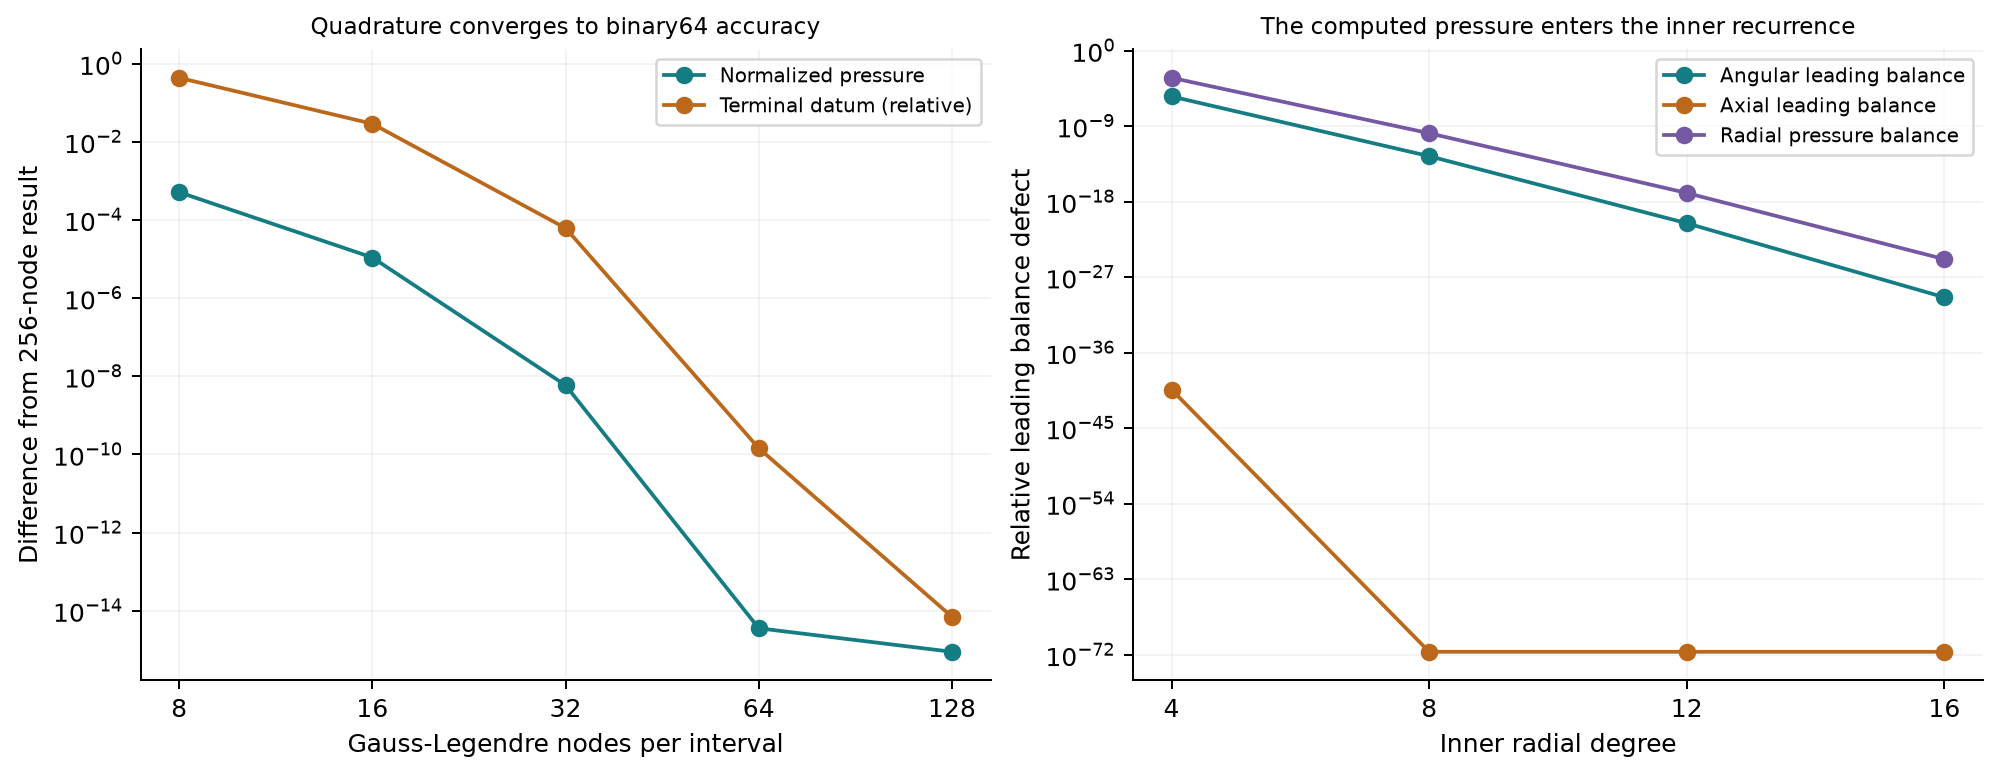
\includegraphics[keepaspectratio,alt={Quadrature differences approach binary64 accuracy, and the inner recurrence\textquotesingle s leading balance defects decrease with radial degree, with the axial balance reaching roundoff.}]{figures/03_pressure_and_handoff_convergence.png}}

}

\caption{\label{fig-convergence}Left: quadrature refinement for the
pressure and terminal target. Right: leading inner balance defects when
the computed pressure supplies the axis data; the axial curve reaches
the working-arithmetic floor. The right panel measures consistency with
the supplied numerical pressure, whose quadrature error is a separate
limitation.}

\end{figure}%

The inner calculation uses 70-digit arithmetic, so its equation defects
can become much smaller than the pressure-input uncertainty. Those tiny
defects do \textbf{not} imply 70-digit accuracy relative to the source's
exact pressure integral. Changing the quadrature from 128 to 256 nodes
changes the computed axial profile by about \textbf{4.5e-18} at the
selected point. The
\href{../../code/d6_axis_pressure/data/handoff_quadrature_change.csv}{propagated-change
table} makes this difference explicit.

\subsection{One joining condition now has a sufficient
bound}\label{one-joining-condition-now-has-a-sufficient-bound}

The earlier analytic test data failed condition (B.2), which requires
\(\chi>0.99\) wherever the axis expression \(Z_*\) is sufficiently
small. For the present pressure we can use its sign and lower-magnitude
bound to confine that region near \(\eta=0\).

With the declared threshold \(\delta=1\), \(|Z_*|\le1\) implies
\(|\eta|\) is at most about \textbf{3.17e-15}. Throughout that band, the
lower bound on \(\chi\) is approximately \textbf{0.999975}.

The lower bound exceeds \(0.99\). The derivation uses the exact initial
pressure contribution and the common sign of the remaining pressure
terms; it does not rely on sampling a very narrow region and hoping to
find its minimum. The \href{source-notes.md}{source notes} give the
algebra.
\href{https://cdn.openai.com/pdf/32d9f210-8b73-45e0-91bc-82a30aef8a9a/navier-stokes.pdf}{OpenAI,
Equation (B.2), page 144, and Equation (A.22), page 133}

This establishes a sufficient bound for that particular condition. The
complex-domain amplitude bound, inner exit inequality, outer stress
cone, annular moment matching, and first correction remain separate
requirements.

We have now replaced the arbitrary pressure test function with a
computed, source-defined schedule datum in a local inner calculation.
The \href{../../code/d6_axis_pressure/study.ipynb}{executed notebook}
reproduces the study, while the
\href{../d6_moment_correction/implementation-ledger.md}{D6 ledger}
records what is still needed for the full corrected flow.




\end{document}
